\documentclass[12pt]{report}
\usepackage[pdftex]{graphicx}
%\usepackage[pdftrex/bookmarksnumbered=true]{hyperref}
\usepackage{hyperref}
\linespread{1.5}
\textwidth = 6in
\textheight = 9in
\usepackage[body={6.0in, 8.2in},left=1.25in,right=1.0in,top=1.0in, bottom=1.0in]{geometry}
\frenchspacing
\usepackage{fancyhdr}
\usepackage{color}
\usepackage{xcolor}
\usepackage{listings}
\lstset{
language=Java,
basicstyle=\small\sffamily,
numbers=left,
numberstyle=\tiny,
frame=tb,
columns=fullflexible,
showstringspaces=false
}

\usepackage{caption}
\DeclareCaptionFont{white}{\color{white}}
\DeclareCaptionFormat{listing}{\colorbox{gray}{\parbox{\textwidth}{#1#2#3}}}
\captionsetup[lstlisting]{format=listing,labelfont=white,textfont=white}


\begin{document}
\pagenumbering{roman}
%\input{Coverpage.tex}

%----------------title page
%\begin{titlepage}
%\begin{center}
%{\bf \large Decision Tree Classifier with GA based feature selection}\\
%\vspace{.15in}
%{\bfseries Mini Project Report}\\
%\vspace{.15in}
%{\normalsize Submitted to} \\
%\vspace{.1in}
%{\bfseries DEPARTMENT OF COMPUTER SCIENCE AND ENGINEERING}\\
%\vspace{.25in}
%{\normalsize \emph{By}}\\
%{\bfseries\normalsize Samir Sheriff }\\
%{\bfseries\normalsize Satvik N }\\
%\vspace{.25in}
%{\normalsize \emph{In partial fulfilment of the requirements\\ for the award of the degree \\
%\vspace{.15in}
%} } 
%
%\vspace{.15in}
%{\large{BACHELOR OF ENGINEERING}}\\
%\vspace{.15in}
%{\normalsize{IN}}\\
%\vspace{.15in}
%{\bfseries\normalsize COMPUTER SCIENCE AND ENGINEERING}\\
%\vspace{0.15in}
%
%\begin{figure}[h!]
%	\centering
%		\includegraphics[scale=0.5]{RVCE.png}
%		
%\end{figure} 
%\vspace{.25in}
%{\bfseries\large R V College of Engineering}\\
%{\normalsize (Autonomous Institute, Affiliated to VTU)}\\
%{\bfseries\normalsize BANGALORE - 560059}\\ 
%{\bfseries\large Jan 2013 - Jun 2013}
%\end{center}
%\end{titlepage}


%---------Declaration
\begin{titlepage}
%\chapter*{\centerline{DECLARATION}}
\begin{center}
\section*{DECLARATION}
\end{center}

\paragraph{}  We, Samir Sheriff and Satvik N bearing USN number 1RV09CS093 and 1RV09CS095 respectively, hereby declare that the dissertation entitled ``\textbf{Decision Tree Classifier with GA based feature selection}'' completed and written by us, has not been previously formed the basis for the award of any degree or diploma or certificate of any other University.
\vspace{1in}

\begin{flushright} {Bangalore \hspace{4.4in} Samir Sheriff } 
 {USN:1RV09CS093}
 \end{flushright}

\begin{flushright} { Satvik N } \\
 {USN:1RV09CS095}
 \end{flushright}
\end{titlepage}

%%---------Certificate
\begin{titlepage}
\newpage
\begin{center}
{\bfseries\large R V COLLEGE OF ENGINEERING}\\
{\normalsize (Autonomous Institute Affiliated to VTU)}\\
{\normalsize DEPARTMENT OF COMPUTER SCIENCE AND ENGINEERING}\\
\end{center}
	
\begin{figure}[h!]
	\centering
		\includegraphics[scale=0.5]{RVCE.png}
		%\includegraphics{msrit-logo.jpg}
	%\caption{}
	%\label{fig:logo2}
\end{figure}

\begin{center}
\bf{\underline{CERTIFICATE}}
\end{center}
\noindent This is to certify that the dissertation entitled, ``\textbf{Decision Tree Classifier with GA based feature selection}'',  which is being submitted herewith for the award of B.E is the result of the work completed by \textbf{Samir Sheriff and Satvik N}  under my supervision and guidance.
\vspace{.5in}

\begin{flushleft} 
\vspace{.5in}
Signature of Guide 	
\hspace{4cm}
 Signature of Head of Department  \\
(Mrs. Shanta R)  \hspace{6cm}(Dr. N K Srinath) \\
 
 \end{flushleft} 
\begin{flushleft}
\hspace{1in}Name of Examiner \hspace{1.25in} Signature of Examiner
\end{flushleft}
\begin{flushleft}
1: \\
\vspace{.5in} 
2: 
\end{flushleft}
\end{titlepage}


%---------Acknowledgement
  
%\linespread{1.5}
\setcounter{page}{1}
\begin{center}
\section*{ACKNOWLEDGEMENT}
\addcontentsline{toc}{section}{ACKNOWLEDGEMENT}
\end{center}
Any achievement, be it scholastic or otherwise does not depend solely on the individual efforts but on the guidance, encouragement and cooperation of intellectuals, elders and friends. A number of personalities, in their own capacities have helped me in carrying out this project work. We would like to take this opportunity to thank them all.

First and foremost we would like to thank Dr. B. S. Satyanarayana, Principal, R.V.C.E, Bengaluru, for his moral support towards completing my project work.

We deeply express my sincere gratitude to our guides Ms. Shanta Rangaswamy, Assistant Professor and Dr. Shobha G, Professor, Department of CSE, R.V.C.E, Bengaluru, for their able guidance, regular source of encouragement and assistance throughout this project. 

We would like to thank Dr. N. K. Srinath, Head of Department, Computer Science \& Engineering, R.V.C.E, Bengaluru, for his valuable suggestions and expert advice.

We thank our Parents, and all the Faculty members of Department of Computer Science \& Engineering for their constant support and encouragement.

Last, but not the least, We would like to thank our peers and friends who provided me with valuable suggestions to improve our project.
\begin{flushright}
Samir Sheriff\\
8th semester, CSE\\
USN:1RV09CS093\\

Satvik N\\
8th semester, CSE\\
USN:1RV09CS095\\

Vaishakh B N\\ 
8th semester, CSE\\
USN:1RV09CS114\\

\end{flushright}

\newpage

%--------------Abstract
%\fontfamily{roman}%\selectfont
\begin{center}
\section*{ABSTRACT}
\addcontentsline{toc}{section}{ABSTRACT}
\end{center} 
A time series is a sequence of data points, measured typically at successive points in time spaced at uniform time intervals. Time series analysis comprises methods for analysing time series data in order to extract meaningful statistics and other characteristics of the data.In the context of statistics,the primary goal of time series analysis is forecasting. In the context of signal processing it is used for signal detection and estimation, while in the context of data mining, pattern recognition and machine learning time series analysis can be used for clustering, classification, query by content, anomaly detection as well as forecasting. This project is aimed making a time series data mining tool which can be used to accomplish the above goals. 

@TODO Data sets names to be added 

The project makes use of quite a few data sets in for time series analysis. these include Rainfall Data from Sita Nadi, electricity consumption data from XYZ city, ECG data and Sea Level Data. Anomaly detection, forecasting, Similarity detection is performed on these data sets using the algorithms available in literature. 

@TODO Key findings and results come here




%------Table Of Contents
\addcontentsline{toc}{section}{CONTENTS}
\tableofcontents

\newpage
\addcontentsline{toc}{section}{LIST OF FIGURES}
\listoffigures

\newpage
\addcontentsline{toc}{section}{LIST OF TABLES}
\listoftables




\newpage

\pagenumbering{arabic}
\setcounter{page}{1}

\pagestyle{fancy}
\lhead{\scriptsize{Introduction}}
\chead{}
\rhead{\scriptsize{Time Series Data Mining Tool}}
\lfoot{\scriptsize{Dept. of CSE, RVCE, Bangalore.}}
\rfoot{\small{\thepage}}
\cfoot{\scriptsize{Jan 2013 - Jun 2013}}
\renewcommand{\headrulewidth}{0.4pt}
\renewcommand{\footrulewidth}{0.4pt}

\chapter{INTRODUCTION}
A time series is a set of observations Xt , each one being recorded at a specific time t. Discrete-time time series is one in which the set T of times at which observations are made is a discrete set. Continuous-time time series are obtained when observations are recorded continuously over some time interval, e.g., when T0 belongs [0,1]. Examples of time series are the daily closing value of the ECG readings and the annual flow volume of the Nile River at Aswan. Time series are very frequently plotted via line charts. Time series analysis comprises methods for analysing time series data in order to extract meaningful statistics and other characteristics of the data. Time series forecasting is the use of a model to predict future values based on previously observed values.  
\section{DEFINITIONS AND USAGE}
Definition of Time Series: An ordered sequence of values of a variable at equally spaced time intervals.
TSDM : Time Series Data Mining tool.
@TODO ADD DETAILS OF THIS SECTION
%-----------------------literature survey--------------------------------------------
\section{LITERATURE SURVEY}
A time series is a collection of observations made sequentially through time. At each time point one or more measurements may be monitored corresponding to one or more attributes under consideration. The resulting time series is called univariate or multivariate respectively. In many cases the term sequence is used in order to refer to a time series, although some authors refer to this term only when the corresponding values are non-numerical. Throughout this paper the terms sequence and time series are being used interchangeably.
The most common tasks of time series data mining methods are: indexing, clustering, classification, novelty detection, motif discovery and rule discovery. In most of the cases, forecasting is based on the outcomes of the other tasks. A brief description of each task is given below.\\
\textbf{Indexing:} Find the most similar time series in a database to a given query time series.\\
\textbf{Clustering:} Find groups of time series in a database such that, time series of the same group are similar to each other whereas time series from different groups are dissimilar to each other.\\
\textbf{Classification:} Assign a given time series to a predefined group in a way that is more similar to other time series of the same group than it is to time series from other groups.\\
\textbf{Novelty detection:} Find all sections of a time series that contain a different behavior than the expected with respect to some base model.\\
\textbf{Motif discovery:} Detect previously unknown repeated patterns in a time series database.\\
\textbf{Rule discovery:} Infer rules from one or more time series describing the most possible behaviour that they might present at a specific time point (or interval).\\
  The temporal aspect of data arises some special issues to be considered and/or imposes some restrictions in the corresponding applications. First, it is necessary to define a similarity measure between two time series and this issue is very important in TSDM since it involves a degree of subjectivity that might affect the final result. A lot of research has focused on defining different similarity measures in order to improve the performance of the corresponding methods. Second, it is necessary to apply a representation scheme on the time series data. Since the amount of data may range from a few megabytes to terabytes, an appropriate representation of the time series is necessary in order to manipulate and analyze it efficiently. The desirable properties that this approach should hold are: 
(a) the completeness of feature extraction 
(b) the reduction of the dimensionality “curse” [1]. 
More specifically, the method of extraction features should guarantee that there would be no pattern missed, the number of patterns falsely identified as interesting will be minimized and the dimensionality reduction will be substantial. In many cases also, the objective is to take advantage of the specific characteristics of a representation that make specific methods applicable (i.e. inducing rules, Markov models). Consequently, the majority of the researchers are focused on defining novel similarity measures and representation schemes in order to improve indexing performance. 
Clustering and classification of time series rely heavily on the similarity measure and the representation scheme selected, thus, there are very few papers proposing a novel algorithm [2]. A recent survey on clustering time series is provided by Liao [3].  
Novelty detection is a very important task in many areas. Several alternative terms for “novelty” have been used, such as, “anomaly”, “interestingness”, “surprising”, “faults” to name a few. Moreover, many problems of finding periodic patterns can be considered as similar problems. The important point here is to provide a clear and concise definition of the corresponding notion. For instance, Keogh et al. [14] describe a pattern as surprising “if the frequency with which it appears, differs greatly from that expected given previous experience”. The authors present a novel algorithm, called Tarzan, and provide useful pointers to relevant literature. Recently, Aref et al. [4] focus on discovering partial periodic patterns in one or more databases. They present algorithms for incremental mining (how to maintain discovered patterns over time as the database is being expanded).
Motif discovery has only recently attracted the interest of the data mining community [9]. Motifs are defined to be previously unknown, frequently occurring patterns in a time series. These patterns may be of particular importance to other data mining tasks, such as, rule discovery and novelty detection. The recent work of Tanaka et al. [7] proposes a new method for identifying motifs from multi-dimensional time series. They apply Principal Component Analysis to reduce dimensionality and perform a symbolic representation. Then, the motif discovery procedure starts by calculating a description length of a pattern based on the “Minimum Description Length” principle.
\begin{itemize}

\item{Indexing }
Indexing approaches are mostly influenced by the pioneer work of Agrawal et al. [1], generalized by Faloutsos et al. [12]. The emerged framework from these papers, referred as GEMINI, can be summarized in the following steps [11]:
•extract k essential features from the time series 
•map into a point in k-dimension feature space
•organize points with off-the-shelf spatial access method.
•discard false alarms
The first and second step suggests the application of a representation scheme in order to reduce the dimensionality. However, this mapping should guarantee that it would return all the qualifying objects. This implies that the similarity measure in the k-dimension feature space should lower bound the corresponding similarity measure in the original space [8]. The third step is an opened selection, however most of the times R-tree structures are used. Other indexing structures may be vp-trees [7] [9], hB-trees and grid-files. The fourth step is a consequence of the fact that this approach can not guarantee that there will not be returned unqualified objects, thus these false alarms should be discarded in a post processing phase.
Recently, Vlachos et al. [8] presented an external memory indexing method for discovering similar multidimensional time series under time warping conditions. The main contribution of this work is the ability to support various distance measures without the need to reconstruct the index. Two approaches with respect to distance measures are taken under consideration, namely, the Longest Common Subsequence (LCS) and the Dynamic Time Warping (DTW). Their indexing technique works by splitting a set of multiple time series in multidimensional Minimum Bounding Rectangles (MBR) and storing them in an R-tree. For a given query, a Minimum Bounding Envelope (MBE) is constructed, that covers all the possible matching areas of the query under time warping conditions. This MBE is decomposed into MBRs and then probed in the R-tree index.
\item{Time series representation}
There have been several time series representations proposed in the literature, mainly on the purpose of reducing the intrinsically high dimensionality of time series. We will refer to some of the most commonly used representations. Discrete Fourier Transform (DFT) [1] was one of the first representation schemes proposed within data mining context. DFT transforms a time series from the time domain into the frequency domain whereas a similar representation scheme, Discrete Wavelet Transform (DWT) [8], transforms it into the time/frequency or space/frequency domain. Singular Value Decomposition (SVD) [5] performs a global transformation by rotating the axes of the entire dataset such that the first axis explains the maximum variance, the second axis explains the maximum of the remaining variance and is orthogonal to the first axis etc. Piecewise Aggregate Approximation (PAA) [3] divides a time series into segments of equal length and records the mean of the corresponding values of each one. Adaptive Piecewise Constant Approximation (APCA) [10] is similar to PAA but allows segments of different lengths. Piecewise Linear Approximation (PLA) approximates a time series by a sequence of straight lines.
Recently, more representation schemes have been proposed in order to reduce dimensionality. The first class of these schemes consists of symbolic representations. Lin et al. [11] propose a Symbolic Aggregate Approximation (SAX) method, which uses as a first step the PAA representation and then discretizes the transformed time series by using the properties of the normal probability distribution. Bagnal[5] assess the effects of clipping original data on the clustering of time series. Each point of a series is mapped to 1 when it is above the population mean and to 0 when it is below. This representation is called clipping and has many advantages especially when the original series is long enough. It achieves adequate accuracy in clustering, it efficiently handles outliers and it provides the ability to employ algorithms developed for discrete or categorical data. Megalooikonomou et al. [30] introduce a novel dimensionality reduction technique, called Piecewise Vector Quantized Approximation (PVQA). This technique is based on vector quantization that partitions each series into segments of equal length and uses vector quantization to represent each segment by the closest codeword from a codebook. The original time series is transformed to a lower dimensionality series of symbols. This approach requires a training phase in order to construct the codebook, a data-encoding scheme and a distance measure.
Cole et al. [9] provide a work that addresses the task of discovering correlated windows of time series (synchronously or with lags) over streaming data. They concentrate in the case where the time series are “uncooperative”, meaning that there does not exist a fundamental degree of regularity that would allow an efficient implementation of DFT  transformations. The proposed method involves a combination of several techniques – sketches (random projections), convolution, structured random vectors, grid structures, and combinatorial design – in order to achieve high performance. Gionis and Mannila [7] introduce a different approach, which is mainly motivated from research on human genome sequences. However, this approach is more general and involves multivariate time series. The notion behind their approach is that, the high variability that some time series very often exhibit, may be explained by the existence of several different sources that affect different segments of this series. More specifically, the task is to find a proper way to segment a time series into k segments, each of which comes from one of h different sources (k >>h). This task is analogous to clustering the points of a time series in h clusters with the additional constraint that a cluster may change at most k-1 times. Gionis and Mannila provide three algorithms for solving this problem and they test them on synthetic and genome data.
Finally, Vlachos et al. [3] propose to represent a time series by applying discrete Fourier transformations and retain the k best Fourier coefficients instead of the first few ones. Although this paper is motivated by mining knowledge from the query logs of the MSN search engine, the proposed methods may be applied for time series data mining in general.
\item{Similarity Measures}
The definition of novel similarity measures has been one of the most researched areas in the TSDM field. Generally, they are strongly related to the representation scheme applied to the original data. However, there are some similarity measures that appear frequently in the literature. Most of the researchers’ choices are based on the family of Lp norms, that include the Euclidean distance. Yi and Faloutsos [3] presented a novel and fast indexing scheme when the distance function is any of the arbitrary Lp norms (p = 1, 2, …, ¥). Another similarity measure that attracted a lot of attention, Dynamic Time Warping (DTW), comes from the speech recognition field [6]. The main advantage of this measure is that it allows acceleration-deceleration of a series along the time dimension (nonlinear alignments are possible), however it is computationally expensive. Markov models have been constructed and experimented. Another family of distance measures, Longest Common Subsequence Measures (LCS), often used in speech recognition and text pattern matching. As an example of this approach, we refer to the work of Agrawal et al. [2] who define two sequences as similar when they have enough, non-overlapping, time-ordered pairs of subsequences that are similar. 
Li et al. [6] propose an algorithm for fast and efficient recognition of motions in multi-attribute continuous motion sequences. The main contribution of this paper is the definition of a similarity measure based on the analysis of Singular Value Decomposition (SVD) properties of similar multi-attribute motions.  The proposed measure deals with noise and takes into account the different rates and durations of each motion. The authors also propose a five-phase algorithm for handling segmentation and recognition in real-time.
Sakurai et al. [5] propose the Fast search method for dynamic Time Warping (DTW) that satisfies the following criteria: 
(a) it is fast 
(b) it produces no false dismissals 
(c) it does not pose any restriction on the series length 
(d) it supports for any, as well as for no restriction on warping scope.
 Their approach is based on a new lower bounding distance measure. They represent the sequence with approximate segments, not necessary of equal length, and operate on them. Three segments, the lower bound, the upper bound, and the time interval, correspond to each one of these approximate segments. In order to fulfill all of the above criteria, they provide algorithms for dynamic programming and searching adjusted to the properties of this representation. Fu et al. [14] propose a new technique to query time series that incorporates global scaling and time warping. The argument is that most real world problems require the ability to handle both types of distortion simultaneously. The approach is to scale the sequence by a bounded scaling factor and also to find nearest neighbor or evaluate range query by applying time warping. The authors provide definitions and proofs of the necessary lower bounds.
Furthermore, there is the expected contribution to defining similarity measures by papers that propose novel representation schemes, since these two tasks are interrelated to each other. 
\end{itemize}
\section{MOTIVATION}
mr. Manju. 
@TODO Add video link here..
\section{PROBLEM STATEMENT}
Make a paper and publish water data everywhere. :/
@TODO add problem statement. 

\section{OBJECTIVE}
The ability to model and perform decision modelling and analysis is an essential feature of many real-world applications ranging from emergency medical treatment in intensive care units to military command and control systems. Existing formalisms and methods of inference have not been effective in real-time applications where trade-offs between decision quality and computational tractability are essential. The objective of this project is to fill the void that exists and help in proper analysis of time varying data.

\section{SCOPE}
The scope of a time series data mining tool is two fold. The first  is to obtain an understanding of the underlying forces and structure that produced the observed data. The second is to 
fit a model and proceed to forecasting, monitoring or even feedback and feed forward control. The time series data mining tool can be used in the following fields. 
\begin{itemize}
\item{\textbf{Economic Forecasting}}
\item{\textbf{Sales Forecasting}}
\item{\textbf{Rainfall Analysis}}
\item{\textbf{Stock Market Analysis}}
\item{\textbf{Yield Projections}}
\item{\textbf{Process and Quality Control}}
\item{\textbf{Census Analysis}}
\end{itemize}
\section{METHODOLOGY}
Time series analysis of data requires the user to able to view the different algorithms and the result obtained from each algorithm along with the graphs which help the user understand the time varying nature of the data. Hence, the representation of data becomes very important. Having understood this requirement in the early phase of the project, we adopted a methodology that will accomplish the objectives in a neat and intuitive way. A GUI was developed in the form of Java Server Pages and the back end was coded in Java which helped us exploit the object oriented paradigm in design of algorithms. 

\section{ORGANIZATION OF REPORT}
@TODO after all chapters are complete.

\pagestyle{fancy}
\lhead{\scriptsize{Software Requirements Specification}}
\chead{}
\rhead{\scriptsize{Decision Tree Classifier with GA-based Feature Selection}}
\lfoot{\scriptsize{Dept. of CSE, R V C E, Bangalore.}}
\rfoot{\small{\thepage}}
\cfoot{\scriptsize{Jan 2013 - Jun 2013}}
\renewcommand{\headrulewidth}{0.4pt}
\renewcommand{\footrulewidth}{0.4pt}

\chapter{SOFTWARE REQUIREMENTS SPECIFICATION}

\paragraph{}Software Requirement Specification (SRS) is an important part of software development process. It includes a set of use cases that describe all the interactions of the users with the software. Requirements analysis is critical to the success of a project. \\

\section{PRODUCT PERSPECTIVE}

\paragraph{} Time Series Data Mining tool is a unique product that makes use of different algorithms to predict, view similarities, and points out the anomalies in different time varying data sets. It is built in a pluggable fashion where the only requirement at the users end is the browser and a working internet connection. 
\section{PRODUCT FEATURES}
\paragraph{} 
The time series data mining tool has many features that distinguishes it from the others available already in the open world. It provides accurate results using the similarity finding, anomaly finding algorithms. The back propagation neural network helps us predicting the future values. On the front end, the user has options to choose the algorithm of her choice. Also, the charts which depict the output are carefully plotted using the google charts API which has been made available by Google Inc. Also, Java beans along with servlets and java server pages and best practices of coding have been followed. 
 
\section{CONSTRAINTS}
\paragraph{}During the development of this product, constraints were encountered. Some specific constraints under which the time series data mining tool has are :

\begin{itemize} 
\item{}Add Constraints
\item{} Add Constraints
\end{itemize}

\section{ASSUMPTIONS AND DEPENDENCIES}
 \begin{itemize}
\item{}It is assumed that the user of this tool has basic understanding of time series data mining.
 
\item{}Also, the user must have a decent knowledge of the interpretation of line graphs.
\end{itemize}

\section{SPECIFIC REQUIREMENTS}
\paragraph{}This section shows the functional requirements that are to be satisfied by the system. All the requirements exposed here are essential to run this tool successfully.

\subsection{FUNCTIONAL REQUIREMENTS}
\paragraph{}The functionality requirements for a system describe the functionality or the services that the system is expected to provide. This depends on the type of software system being developed. 
The requirements that are needed for this project are :
 \begin{itemize}
\item The data sets should be normalized so that the algorithms can be applied effectively.
\item A good representation of the results should be made available to the users through proper representation media like graphs.
\end{itemize}
 \begin{itemize}
\item TODO ADD SOMETHING HERE.
\end{itemize}
\subsection{SOFTWARE REQUIREMENTS}
\subsubsection{DEVELOPERS MACHINE}
\begin{itemize}
\item{	Operating System: Windows 7/8, Linux, Mac}
\item{  Software Tools : Java, JDK 7.0, Apache Tomcat Server version 7.0\\ Web Browser (Mozilla, IE8+, Chrome)} 
\item {IDE : Eclipse IDE for J2EE Developers}
\item {API Libraries : }JQuery UI and Ajax Libraries (Active Internet Connection)

\end{itemize}
\subsubsection{END USERS MACHINE}
\begin{itemize}
\item {Java Enabled Browser }
\item { Active Internet Connection }
\end{itemize}
\subsection{HARDWARE REQUIREMENTS}
\begin{itemize}
\item{Processor: Intel Pentium 4 or higher version}
\item{RAM: 512MB or more}
\item{Hard disk: 5 GB}
\end{itemize}
\subsubsection{SOFTWARE INTERFACES }
The Java Runtime Environment (JRE) is required to run the software.
\pagestyle{fancy}
\lhead{\scriptsize{Decision Tree Learning}}
\chead{}
\rhead{\scriptsize{Decision Tree Classifier with GA-based Feature Selection}}
\lfoot{\scriptsize{Dept. of CSE, RVCE, Bangalore.}}
\rfoot{\small{\thepage}}
\cfoot{\scriptsize{Jan 2013 - Jun 2013}}
\renewcommand{\headrulewidth}{0.4pt}
\renewcommand{\footrulewidth}{0.4pt}
\chapter{HIGH LEVEL DESIGN}
\paragraph{}The software development usually follows Software Development Life Cycle (SDLC). The second stage of SDLC is the design phase. The design stage involves two substages namely High level design and Detailed level design.\\
\paragraph{} High level design gives an overview of how the system works and top level components comprising the system.

\section{SYSTEM ARCHITECTURE}
\paragraph{}This section provides an overview of  the functionality and the working of the time series data mining tool. The overall functionality of the application is divided into different modules in an efficient way. The system architecture is shown in Figure 3.1
\paragraph{}

\begin{figure}[h!]
	\centering
		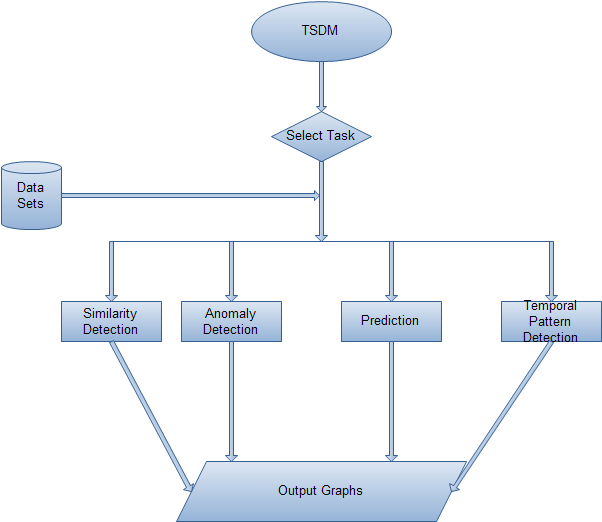
\includegraphics[scale=0.7]{system-architecture.png}
		\caption{System Architecture}
\end{figure} 

\section{DATA FLOW DIAGRAMS}
\paragraph{}A DFD is a figure which shows the flow of data between the different processes and how the data is modified in each of the process. It is very important tool in software engineering that is used for studying the high level design.\\
\paragraph{}There are many levels of DFDs. Level 0 gives the general description and level 1 gives the detailed description. Going higher in the level numbers greater description of the processes will be given.
\pagebreak
\subsection{DFD LEVEL 0}
\paragraph{}The level 0 DFD is shown in Fig. 3.2 below ehich gives the general operation of the steganographic system There are three major components. Two external entities called sender and receiver and one major system called the steganographic system.
\begin{itemize}
\item Sender : The sender is the one responsible to send the data to the receiver. The data to be sent is hidden using the Steganography system. The data is hidden in an image.
\item Receiver : The receiver receives the data that is sent to him in the embedded format. The receiver then extracts the data from the embedded format to get the actual data. The receiver makes use of the Steganography system to extract the data.
\item Steganography System : This the software which is used to embed the data into the image and also to extract the data from the image.
\end{itemize}
%\begin{figure}[h!]
%	\centering
%		\includegraphics[scale=0.8]{level0.jpg}
%		\caption{Data Flow Diagram Level 0}
%\end{figure} 
\pagebreak
\subsection{DFD LEVEL 1}
\paragraph{}There are two major processes in level 1 DFD as shown in Figure 3.3. The processes invloved in here are :
\begin{itemize}
\item Data Embedding: This process represents the actual embedding the data. The inputs given to this process are the data files, cover image. Input image is where the data is to be embedded and the key must also be shared between the sender and the receiver.
\item Data Extraction: This process is used to extract the data back from the stego image. This is the reverse process of embedding. Here the input is the stego image and the key.
\end{itemize}
%\begin{figure}[h!]
%	\centering
%		\includegraphics[scale=0.8]{level1.jpg}
%		\caption{Data Flow Diagram Level 0}
%\end{figure}
\pagebreak
\subsection{DFD LEVEL 2}
\subsubsection{Embedding Phase}
The major processes in Level 2 DFD of Embed process on the sender side are shown in Figure 3.4.
\begin{itemize}
\item Data Holder: Data holder contains all the data bits, which upon invocation will give the required number of bits of data need to be embedded.
\item Pixel Retriever: This retrieves the individual pixels from the cover image. 
\item Processor: Takes the key as the input, encrypts the data and embeds it into the pixels received from the retriever. 
\item A final image is formed as a result of this process.
\end{itemize}
%\begin{figure}[h!]
%	\centering
%		\includegraphics[scale=0.8]{level2-embed.jpg}
%		\caption{Data Flow Diagram Level 2: Embedding}
%\end{figure}
\pagebreak
\subsubsection{Extraction Phase}
\paragraph{}The major processes in the Level 2 DFD of the Extraction module on the receiver side is shown in Figure 3.5. 
\begin{itemize}
\item Data Retriever: The data retriever module extracts the data file from the morphed image which it receives. The key should be present for proper retrieval.
\item Pixel Retriever: Retrieves the pixels from the morphed image and pprovides it to the Data Retriever.
\end{itemize}
%\begin{figure}[h!]
%	\centering
%		\includegraphics[scale=0.8]{level2-extract.jpg}
%		\caption{Data Flow Diagram Level 2: Embedding}
%\end{figure}
\pagebreak

\chapter{DETAILED DESIGN}
\pagestyle{fancy}
\lhead{\scriptsize{Detailed Design}}
\chead{}
\rhead{\scriptsize{Key Based Data Embedding Technique in Image Steganography}}
\lfoot{\scriptsize{Dept. of CSE, R V C E, Bangalore.}}
\rfoot{\small{\thepage}}
\cfoot{\scriptsize{September 2012 - January 2013}}
\renewcommand{\headrulewidth}{0.4pt}
\renewcommand{\footrulewidth}{0.4pt}
\section{STRUCTURED CHART}
\paragraph{}Structure charts are used to specify the high level design or architecture of a computer program. As a design tool, they help the programmer in dividing and conquering a large software problem, i.e. recursively breaking a problem down into parts that are small enough to be understood by a human brain. The process is called top-down design or functional decomposition. 
\paragraph{}Programmers use a structure chart to build a program in a manner similar to how an architect uses a blueprint to build a house. In the design stage, the chart is drawn and used as a method for the client and various software designers to communicate. During the actual building of the program, the chart is continuously referred to as master plan. Often, it is modified as programmers learn new details about the program. After a program is completed, the structured chart is used to fix bugs and to make changes.
\paragraph{} The entire program starts with user entering his choice of input as to either embed or extract. Based on this, the GUI module responds appropriately with success or failure. The digital media chosen by user is taken as input for embedding phase. The digital media is encrypted using AES algorithm before embedding to stego image.This encrypted data is embedded onto image using embedding algorithm to get the stego image containing secret data. A key is generated using Diffie Hellman Key exchange which acts as the input for the embedding algorihm.
\paragraph{} At the receiver end, the Diffie Hellman key is generated once again. From the stego images, secret data is extracted. It will be in encrypted form. The original input data is extracted by using decompression module of AES algorithm. This gives the hidden file's original content.
%\pagebreak

\pagebreak
\section{MODULES DESCRIPTION}
This section describes the main modules that are used in developing the project. This will help us in understanding the working of individual components. 
\subsection{GUI MODULE}
\subsubsection{Definition:} 
\paragraph{} This module is the core module which takes the users input to decide upon which operation to be performed. Based upon user choice, the necessary inputs will be taken in this module. If any errors are generated during any operation, then suitable report is displayed to the user.
\subsubsection{Resources:} 
\paragraph{}The input files are bitmap images and are chosen to embed data. A session key is generated using Diffie Hellman protocol. Also, the data file to be hidden is taken.
\subsubsection{Functionality:} 
\paragraph{}This is the main flowchart which shows all the functions provided by the software. In the beginning, the user is given two options, according to which the user either embeds extracts or exits from the application. This is shown in the decision symbol. According to the decision taken, the operations are performed. If the user chooses to embed, then the functions to select cover image, the secret data, and key generation are performed. Before embedding the secret data encryption is done. After performing these operations, the stego images are sent to the receiver using any wireless medium or LAN. At the receivers end, the receiver implements the functions to extract stego image values, extract secret digits data. After the implementation of these functions, if the user wants to exit from the software, that particular option is also provided to the user. This is shown in Fig 4.2.
%\pagebreak
%\begin{figure}[h!]
%	\centering
%		\includegraphics[scale=0.9]{2.jpg}
%		\caption{GUI Module}
%\end{figure} 
\pagebreak

\pagebreak
%\begin{figure}[h!]
%	\centering
%		\includegraphics[scale=0.9]{7.jpg}
%		\caption{Data Extraction Module}
%\end{figure} 
\pagebreak

\chapter{IMPLEMENTATION}
\pagestyle{fancy}
\lhead{\scriptsize{Implementation}}
\chead{}
\rhead{\scriptsize{Key Based Data Embedding Technique in Image Steganography}}
\lfoot{\scriptsize{Dept. of CSE, R V C E, Bangalore.}}
\rfoot{\small{\thepage}}
\cfoot{\scriptsize{September 2012 - January 2013}}
\renewcommand{\headrulewidth}{0.4pt}
\renewcommand{\footrulewidth}{0.4pt}
\paragraph{}The implementation phase of any project development is the most important phase and yields the final solution which solves the problem at hand.The implementation phase involves the actual materialization of the ideas, which are expressed in a suitable programming language. The factors concerning the programming language selection and platform chosen are described in the following sections.
\section{PROGRAMMING LANGUAGE SELECTION}

\paragraph{}The programming language chosen must reflect the necessities of the project to be completely expressed in terms of the analysis and the design documents. Therefore before choosing the language, features to be included in the project are decided. The time series data mining project needs the following features in a language to be implemented. Some of the features required are stated as follows:
\begin{itemize}
\item J2EE provides us with servlets and JSP which help in dynamically constructing web pages.
\item J2EE provides us with Java Beans which help in proper data manipulation.
\item JSP and servlets make use of Java backend in a very optimal manner. They have special tags which help us exploit these features.
\item Java's core classes are designed from scratch to meet the requirements of an object oriented system.
\end{itemize} 
With these necessities in mind, J2EE is selected as the optimal programming language to implement the project.
\section{PLATFORM}
\paragraph{}The TSDM tool was built and designed on Windows Operating system family. They were specifically tested on Windows 7 with Google Chrome and Mozilla Firefox browsers. Because the product is browser based, any user with the broswers mentioned above will be able to run the tool. The product is hence platform independent in the true sense.
\section{CODE CONVENTIONS}
\paragraph{}The code standards for the Java programming Language document contains the standard conventions that follows. It includes file names, file organizations, indentation, comments, declarations, naming conventions and programming practices. Code conventions improve the readability of the software.
\subsection{Naming Conventions}
@TODO Add shitty things here
\subsection{File Organization}
@TODO Add shitty things here
\subsection{Class Declarations}
@TODO Add shitty things here
\subsection{Comments}
@TODO Add shitty things here
\section{DIFFICULTIES ENCOUNTERED AND STRATEGIES USED TO TACKLE}

\paragraph{}There were a number of challenges that were faced while implementing the Time Series Data Mining tool.Some challenges were challenging and ended up in helping us think innovatively and come up with efficient solutions. Some major problems that were encountered have been stated in brief along with their solutions.
\subsubsection{Problem 1}
\paragraph{}Initially we wanted to build the front end in python using django web framework. But integrating java (back-end) with python had performance issues.(Using Jython interpreter)
\subsubsection{Solution}
\paragraph{}We used JSP (Java server pages) for the front end and solved this problem.
\subsubsection{Problem 2}
\paragraph{}In the initial stages of the project charts4j libraries were used to plot graphs. There were some internal problems with the URL rendering.

\subsubsection{Solution}
\paragraph{}This Problem was solved later by making use of Google's Charts API and java script. 
\subsubsection{Problem 3}
\paragraph{}Initially only Samir was doing the project and We had no clue what was going on.(Need to remove this)
\subsubsection{Solution}
\paragraph{}We gave him a time out and everything became alright! 
\pagebreak






\pagestyle{fancy}
\lhead{\scriptsize{Software Testing}}
\chead{}
\rhead{\scriptsize{Time Series Data Mining Tool}}
\lfoot{\scriptsize{Dept. of CSE, RVCE, Bangalore.}}
\rfoot{\small{\thepage}}
\cfoot{\scriptsize{Jan 2013 - Jun 2013}}
\renewcommand{\headrulewidth}{0.4pt}
\renewcommand{\footrulewidth}{0.4pt}
\chapter{Software Testing}
Introduction to Testing (From wiki)
\section{Test Environment}
Talk about the server environment. 
Server capabilities (No of requests it can process, computation requirements)
\subsection{Unit Testing of Data Center Management Model}

\subsection{Unit Testing of Metrics Adapter and Analyzer Module}
\subsection{Unit Testing of Actuator Module}

\section{Integration Testing of the Modules}
\subsection{Integration of Data Center Management Model Service with Workload Metric Generator}
\subsection{Integration of Metrics Adapter and Analyzer with Workload Metric Generator}
\subsection{Integrate Actuator service with RTIM software}
\section{System Testing}
\section{Functional Testing of the GUI}
\subsection{Design Data Center Resources Artifacts}
\subsection{Design Business Services Artifacts}




\pagestyle{fancy}
\lhead{\scriptsize{Experimental Analysis and Results}}
\chead{}
\rhead{\scriptsize{Time Series Data Mining Tool}}
\lfoot{\scriptsize{Dept. of CSE, RVCE, Bangalore.}}
\rfoot{\small{\thepage}}
\cfoot{\scriptsize{Jan 2013 - Jun 2013}}
\renewcommand{\headrulewidth}{0.4pt}
\renewcommand{\footrulewidth}{0.4pt}
\chapter{Experimental Analysis and Results}
Satvik will do this
\section{Evaluation Metric}
Satvik will do this
\section{Experimental Dataset}
Satvik will do this
\section{Performance Analysis}
Satvik will do this
\section{Inference from the Results}
Satvik will do this



\pagestyle{fancy}
\lhead{\scriptsize{Conclusion}}
\chead{}
\rhead{\scriptsize{Time Series Data Mining Tool}}
\lfoot{\scriptsize{Dept. of CSE, RVCE, Bangalore.}}
\rfoot{\small{\thepage}}
\cfoot{\scriptsize{Jan 2013 - Jun 2013}}
\renewcommand{\headrulewidth}{0.4pt}
\renewcommand{\footrulewidth}{0.4pt}
\chapter{CONCLUSION}
\section{Summary}
In this project, we were able to successfully implement the Time Series Data Mining Tool for analyzing the time series and test its performance. This tool mainly contains four modules, they are - \textbf{Similarity Detection, Forecasting and Prediction, Anomaly Detection and Temporal Pattern Finder}, which we were successful in implementing and testing. The results obtained were presented in the previous chapter.

The description of the modules are below :
\begin{itemize}
\item \textbf{Similarity Detection} : This module helps in finding similarity patterns (that occur at regular intervals in case of periodic time series), comparing different time series data. SAX and DTW are the main algorithms implemented/used in this module.
\item \textbf{Forecasting and Prediction} : This module contain algorithms/models which can be trained from the past time series data and can be used to predict the future values of a time series. 
\item \textbf{Anomaly Detection} : This module contains algorithms that help in indicating anomalous patterns in the time series data analyzed. Anomalies are patterns in time series which deviate from the normal behavior and can indicate fraud/danger depending on the application. For example in an industry which produces the blades, the thickness of the blade can be monitored by a machine as a time series and any deviation from the normal error rate can signal an error in the manufacturing process.
\item \textbf{Temporal Pattern Finder } : This module helps in finding hidden temporal patterns in a time series. This module can be further extended to implement clustering techniques.
\end{itemize}


Initially this project mainly focused on analyzing the sea and water level time series. Later this application was extended to any uni-variate time series data. Users can upload the time series data to be analyzed and get the results instantly. Major data sets used were :
\begin{itemize}
\item Sea Level Dataset : Indicating the sea level at various times of a day.
\item Water Level : Ground Water level data, indicating the ground water level during various moths of an year for upto 5 years.
\item Finance Dataset : Consisting of stock index values of  Nifty and Vix collected every minuted for a week.(5 days,during market hours).
\item ECG Dataset : The ECG  voltage values of patients collected every 4ms.(for 10 patients).
\end{itemize}


In this project, we also analyzed the efficiencies of different algorithms for the same tasks and also compared the results for different data sets.Clearly more work needs to be done.(End this section Properly Boys)


\section{Limitations}
Some of the shortcomings in our project are :
\begin{enumerate}

\item{} The application hangs when analyzing very large data sets (more than 500 MB).
\item{} The application does not support multi-variate time series.
\item{}Some algorithms efficient for a particular data set and may not be efficient for other data set. So user intervention is required in selecting an algorithm for a data set.
\end{enumerate}

\section{Future enhancements}
Some of the future enhancements are :
\begin{enumerate}
\item{The size of the  time series data analyzed is in terms of Mega Bytes. For larger dataset(In terms of GBs) or big data, distributed computing technologies like Hadoop can be used.}
\item{}The application can be extended to analyze multi variate time series data.
\item{The application could be made more responsive by using Threads and Parallel/Cloud Computing}
\item{One more extension could be analyzing twitter post data with respect to time and predicting the trends. This requires NLP, but is an example of time series.}
\item{Efficient algorithms using Support Vector Models (SVMs) for forecasting, Hidden Markov Model for anomaly detection can be implemented.}
\item{This application uses static time series data, enhancements can be made to use real time data.(In finance applications)}

\item{This application can be converted into an mobile application (android, iPhone, iPad) where the users can analyze the time series data on the go and share the results on facebook}
%--- For efficient page utilization!
% Currently only classification accuracy is returned.
%However, there is potentially exploitable information with
%respect to which features were actually used to build the
%decision tree and their relative positions in the tree.
\end{enumerate}



%For Bib refer to refs.bib to add/remove bib items
\addcontentsline{toc}{section}{BIBLIOGRAPHY}
\begin{thebibliography}{refs}
\bibitem{test}Agrawal R., Lin K.-I., Sawhney H. S., Shim K.,\textit{“Fast Similarity Search in the Presence of Noise,Scaling, and Translation in Time-Series Databases”}
\bibitem{t}Genetic Algorithm for constructing DT - \url{http://www.jprr.org/index.php/jprr/article/viewFile/44/25}
\bibitem{te}Decision Trees - \url{http://web.cecs.pdx.edu/~mm/MachineLearningWinter2010/pdfslides/DecisionTrees.pdf}
\bibitem{t} Project brief for the DT  using Horse data sets  - \url{https://cs.uwaterloo.ca/~ppoupart/teaching/cs486-spring06/assignments/asst4/asst4.pdf}
\bibitem{t}Supervised and Unsupervised Discretization of Continous Features - \url{http://robotics.stanford.edu/users/sahami/papers-dir/disc.pdf}
\bibitem{t}Hybrid learning using Genetic Algorithms and Decision Trees for pattern sification - \url{http://cs.gmu.edu/~eclab/papers/ijcai95.pdf}
\bibitem{t}Kardi Tutorials on Decision Trees- \url{http://people.revoledu.com/kardi/tutorial/DecisionTree/index.html}


%\bibitem{}
%\bibitem{}
\end{thebibliography}

\newpage
\pagestyle{fancy}
\lhead{\scriptsize{Appendix A: Source Code}}
\chead{}
\rhead{\scriptsize{Time Series Data Mining Tool}}
\lfoot{\scriptsize{Dept. of CSE, RVCE, Bangalore.}}
\rfoot{\small{\thepage}}
\cfoot{\scriptsize{Jan 2013 - Jun 2013}}
\renewcommand{\headrulewidth}{0.4pt}
\renewcommand{\footrulewidth}{0.4pt}

\addcontentsline{toc}{section*}{APPENDICES}
\section*{Appendices}
\section*{Appendix A : Source Code}

%\lstinputlisting[language=Java, caption=DecisionTreeConstructor.java, breaklines=true]{../../src/org/ck/dt/DecisionTreeConstructor.java}
%\lstinputlisting[language=Java, caption=DecisionTreeClassifier.java, breaklines=true]{../../src/org/ck/dt/DecisionTreeClassifier.java}


\newpage
\pagestyle{fancy}
\lhead{\scriptsize{Appendix B: Screen shots}}
\chead{}
\rhead{\scriptsize{Time Series Data Mining Tool}}
\lfoot{\scriptsize{Dept. of CSE, RVCE, Bangalore.}}
\rfoot{\small{\thepage}}
\cfoot{\scriptsize{Jan 2013 - Jun 2013}}
\renewcommand{\headrulewidth}{0.4pt}
\renewcommand{\footrulewidth}{0.4pt}


\section*{Appendix B : Screen Shots}
\begin{figure}[h!]

  \centering
    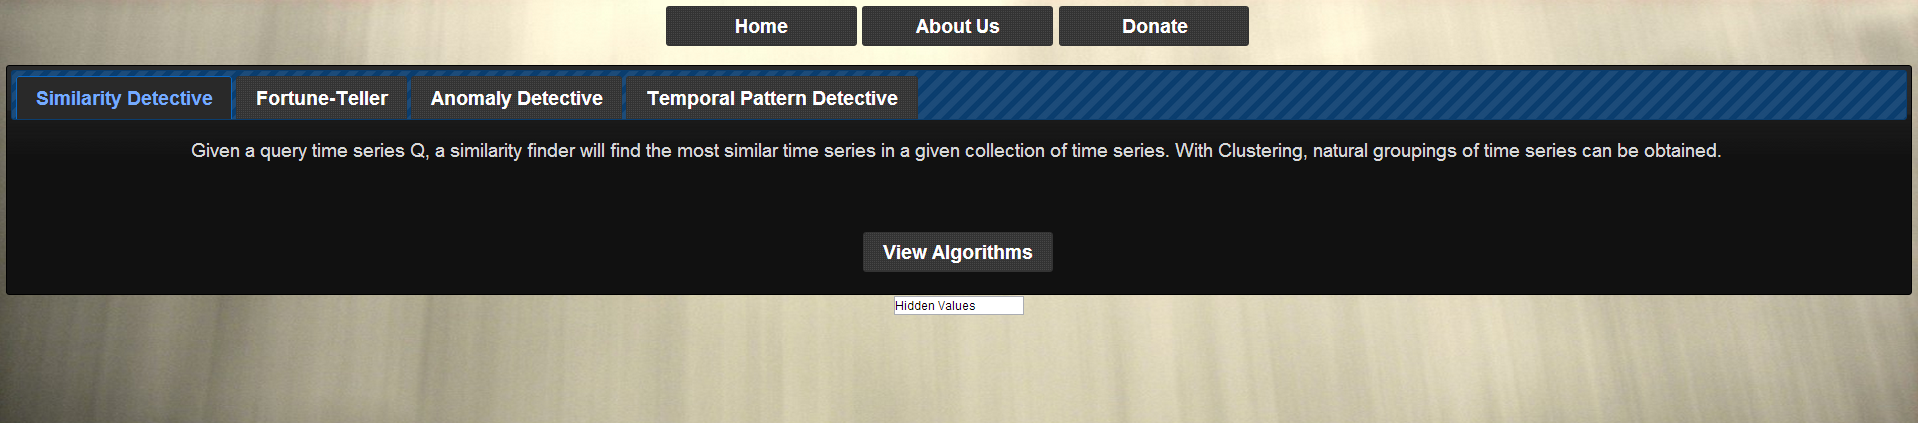
\includegraphics[scale=0.35]{./screenshots/welcome_screen.png}
  \caption{TSDM Tool Window - Welcome Screen}
\end{figure}

\begin{figure}[h!]
  
  \centering
    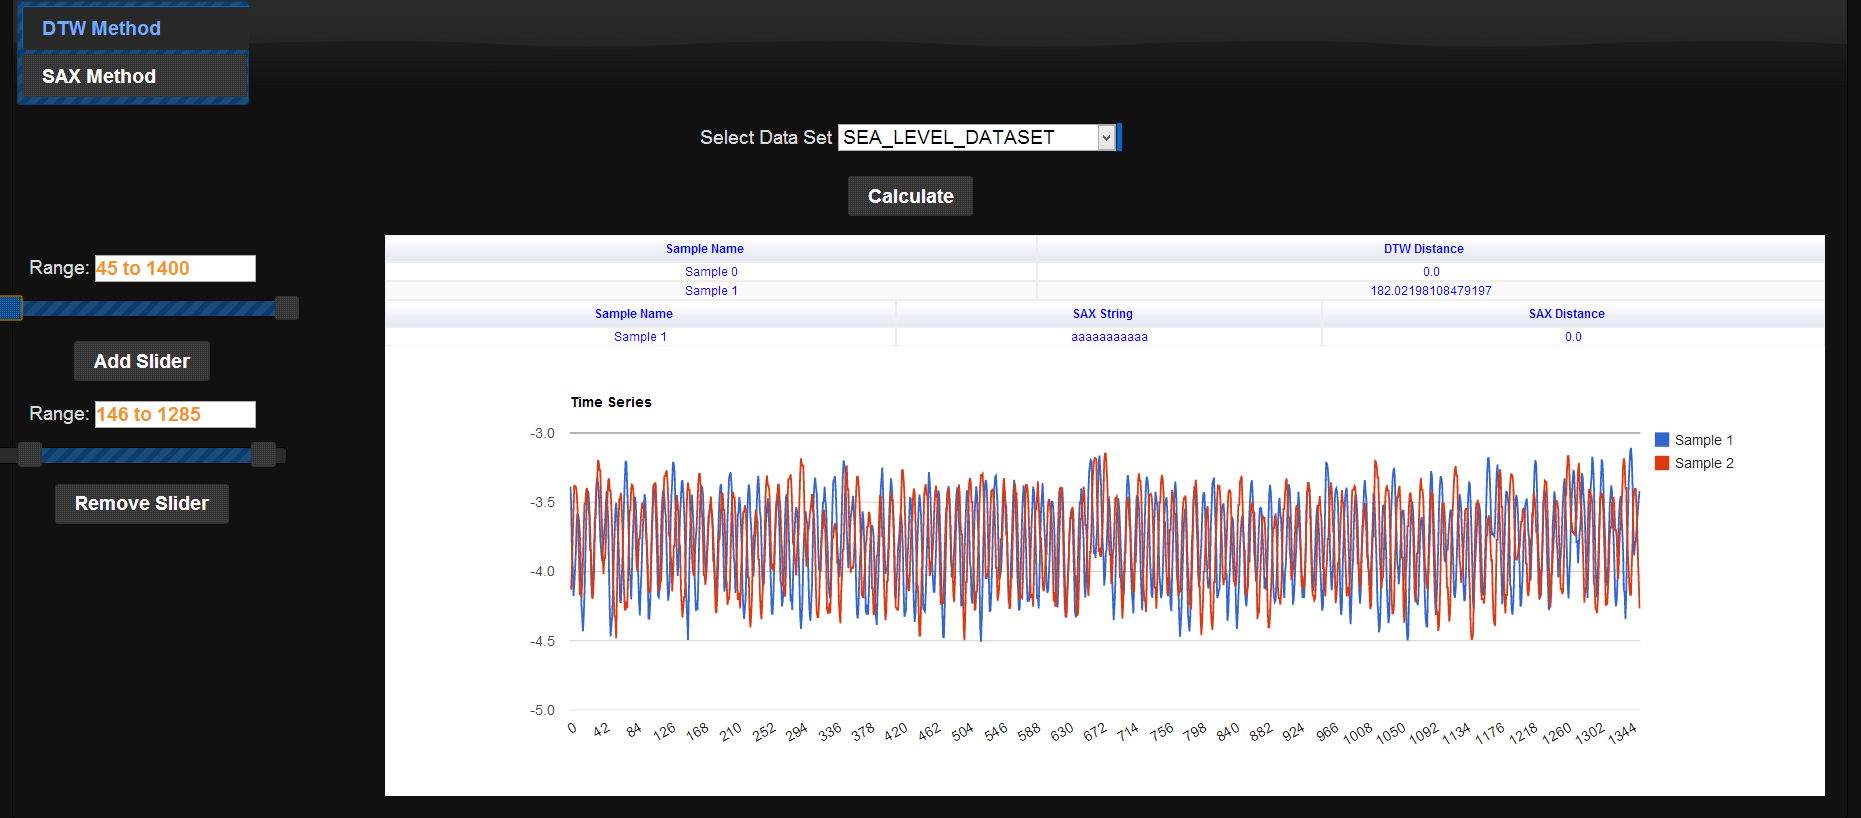
\includegraphics[scale=0.35]{./screenshots/sim_dtw.png}
\caption{Similarity Detection with DTW Algorithm.}
\end{figure}

\begin{figure}[h!]
  
  \centering
    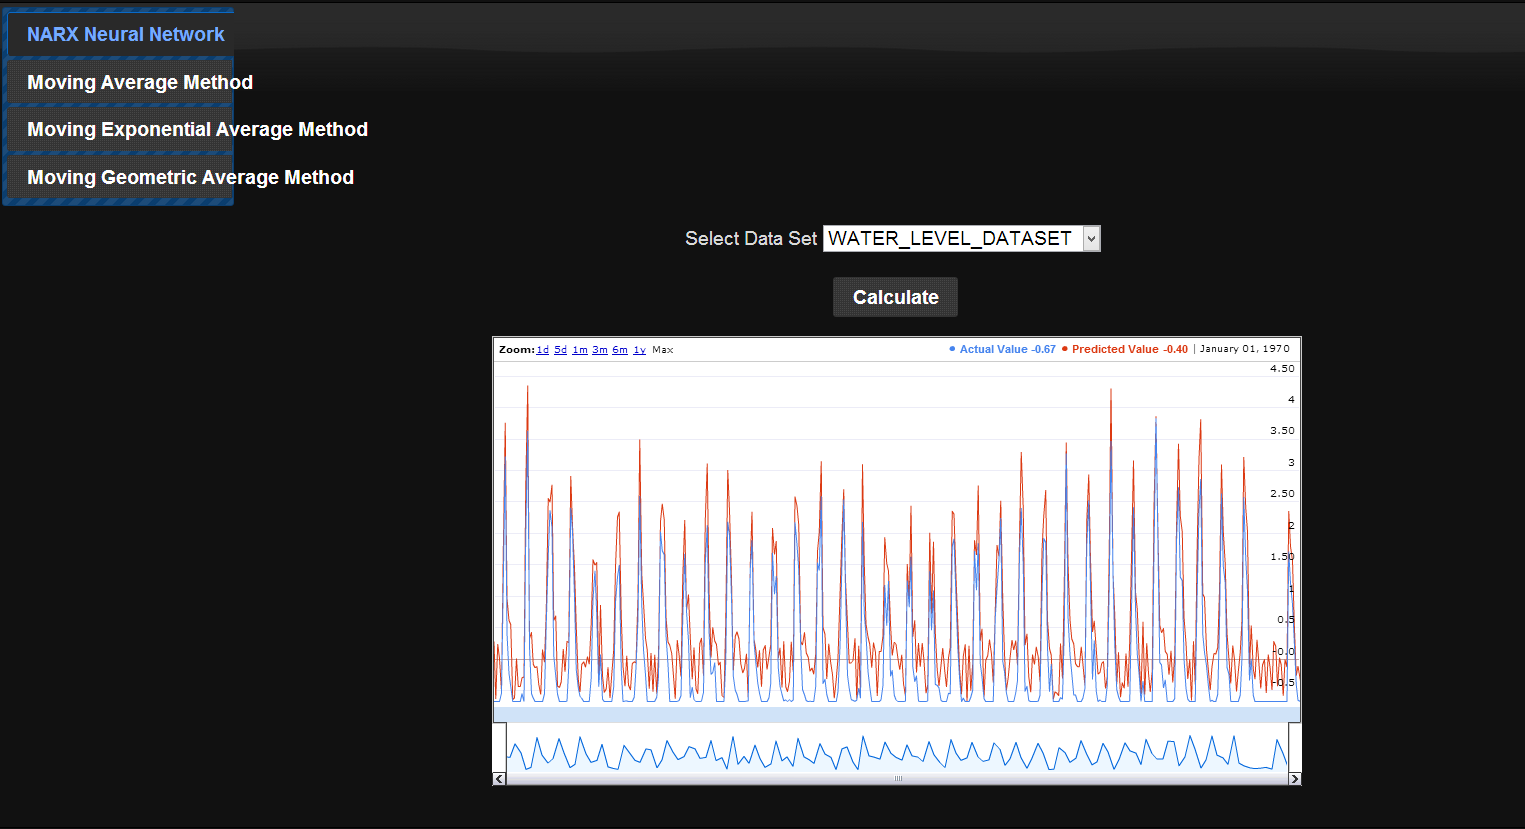
\includegraphics[scale=0.40]{./screenshots/ft_narx.png}
\caption{Time Series Prediction with NARX NN Model.}
\end{figure}
\begin{figure}[h!]
  
  \centering
    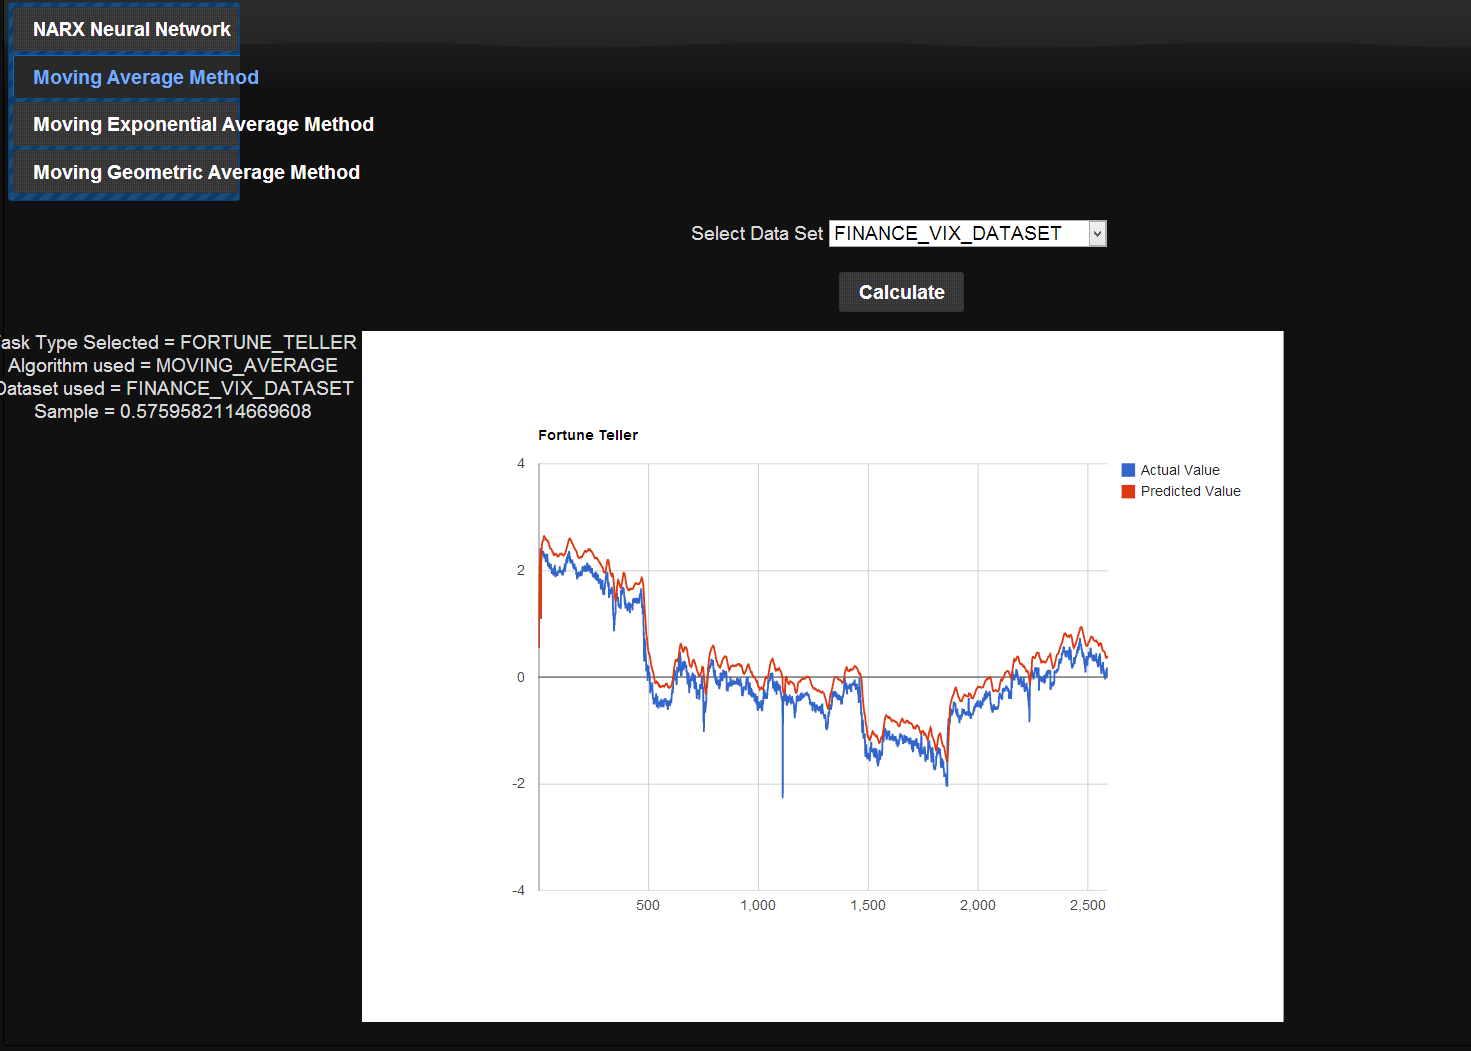
\includegraphics[scale=0.400]{./screenshots/ft_mv_avg.png}
\caption{Time Series Prediction with Moving Average Method.}
\end{figure}

\begin{figure}[h!]
  
  \centering
    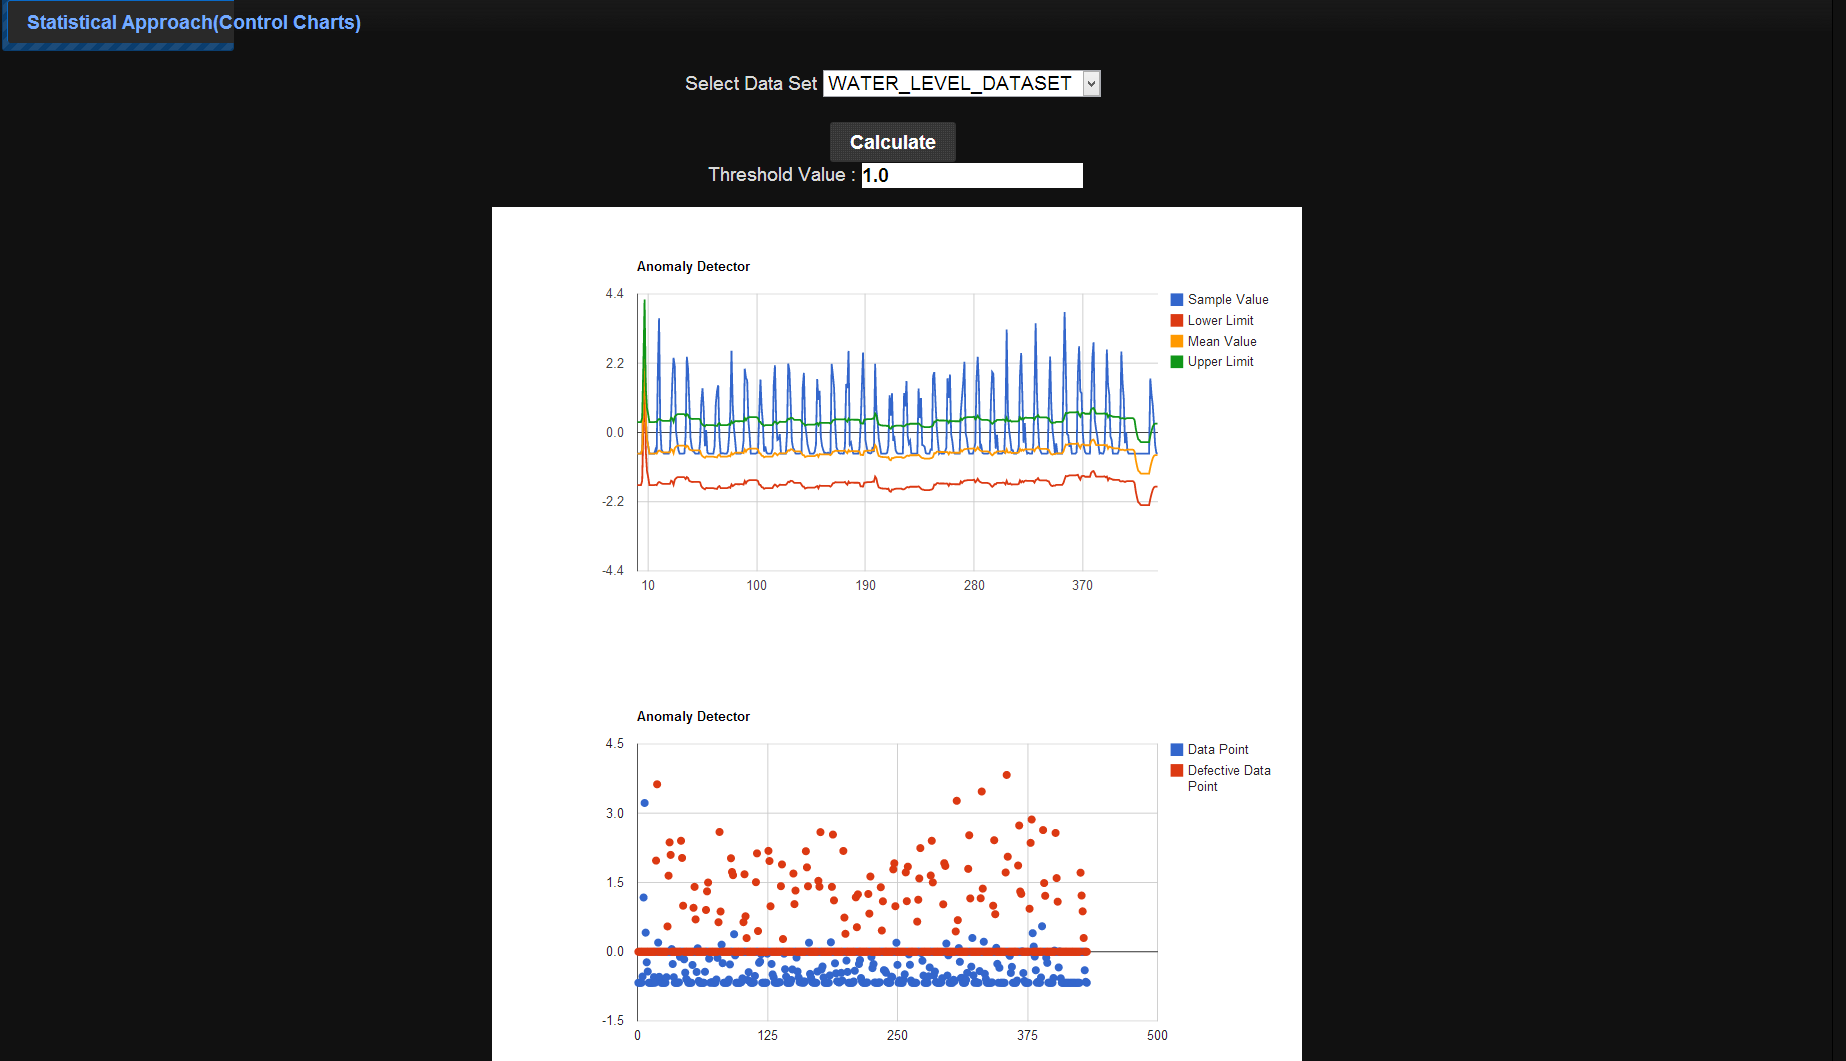
\includegraphics[scale=0.350]{./screenshots/ano_stat_app.png}
\caption{Anomaly Detection using Statistical Approach.}
\end{figure}

\begin{figure}[h!]
  
  \centering
    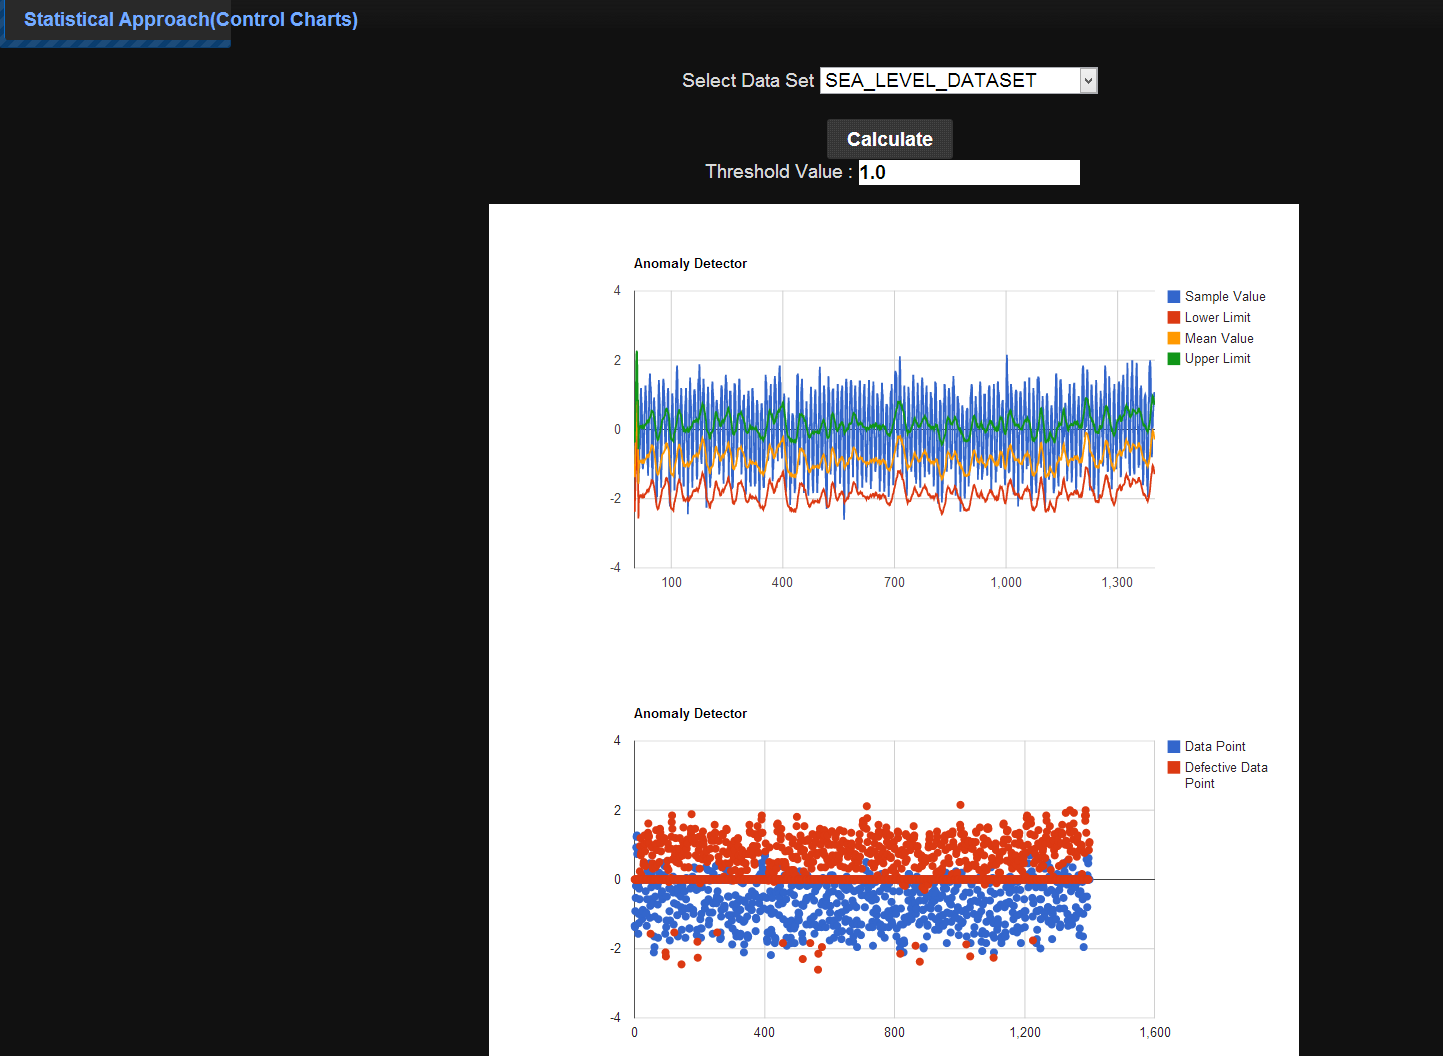
\includegraphics[scale=0.350]{./screenshots/ano_stat_app_2.png}
\caption{Anomaly Detection using Cusum Algorithm.}
\end{figure}

\begin{figure}[h!]
  
  \centering
    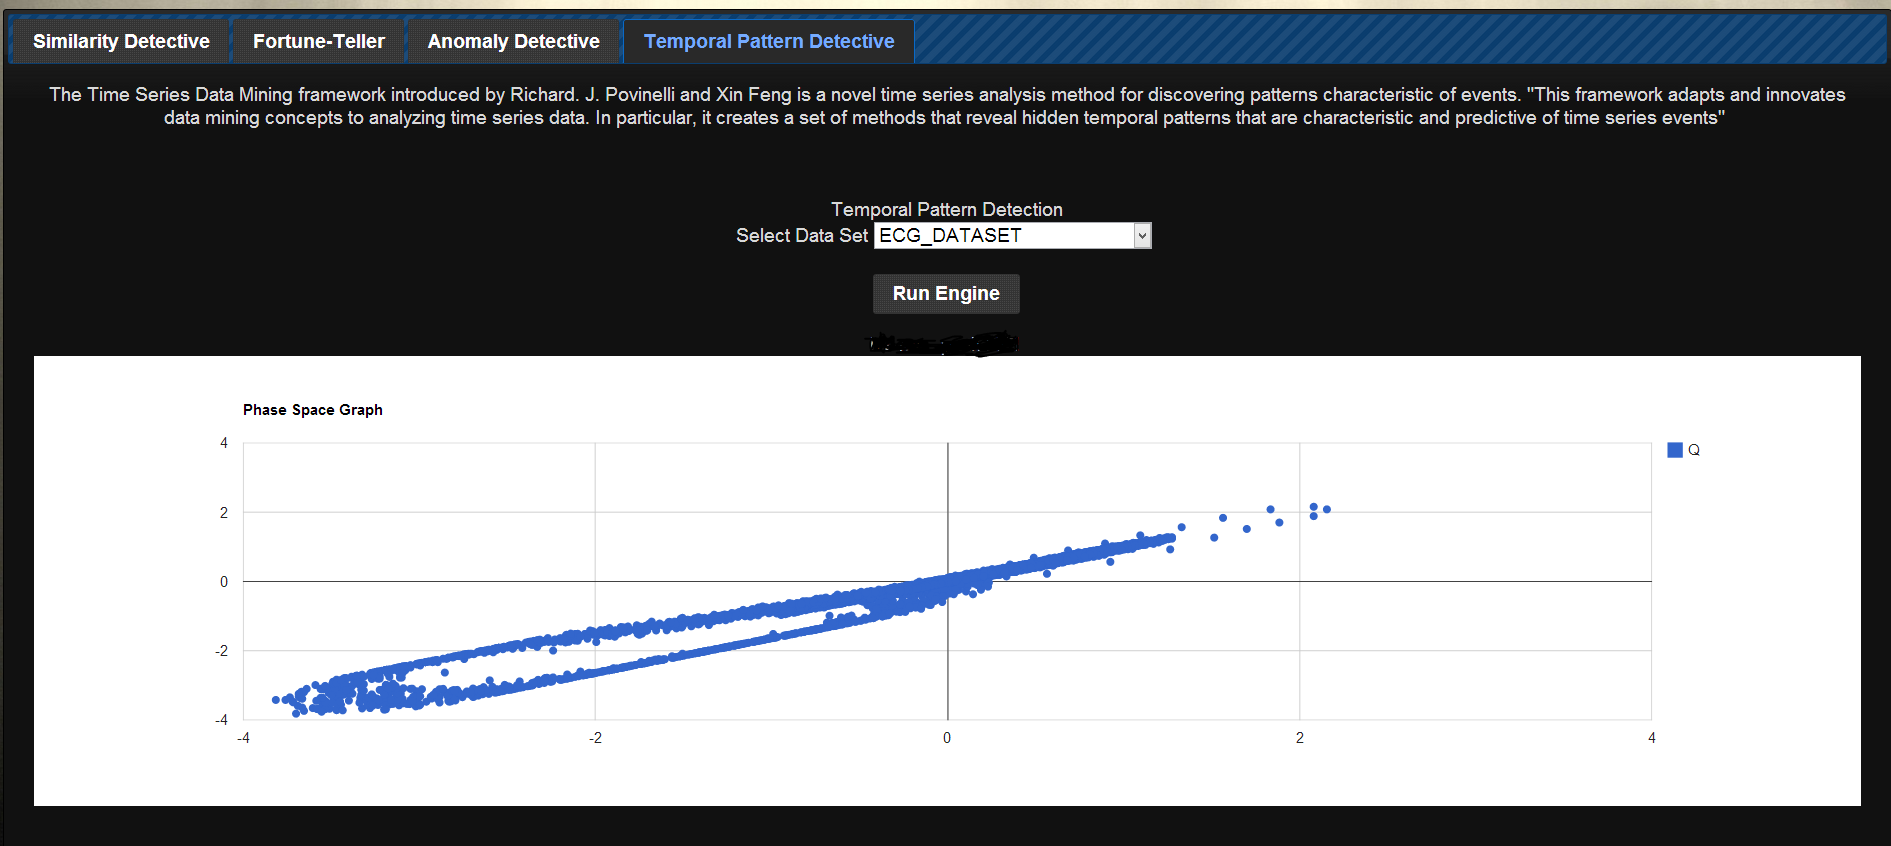
\includegraphics[scale=0.350]{./screenshots/temp_pattern.png}
\caption{Anomaly Detection using Cusum Algorithm.}
\end{figure}
\begin{figure}[h!]
  
  \centering
    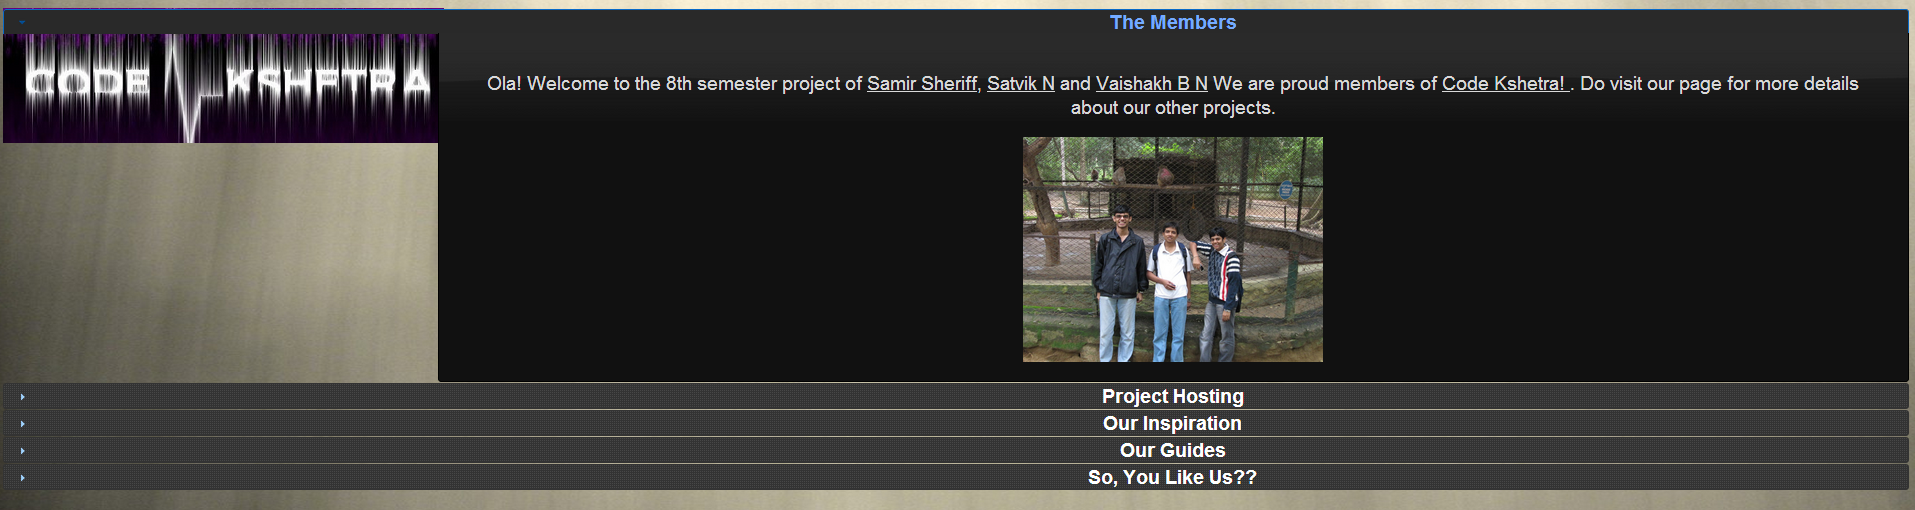
\includegraphics[scale=0.35]{./screenshots/about_us.png}
\caption{About the Developers who did this project!}
\end{figure}

\end{document}
